\documentclass[11pt]{article}

\usepackage[a4paper,margin=18mm]{geometry}
\usepackage{amsmath,amssymb}
\usepackage{array}
\usepackage{booktabs}
\usepackage{graphicx}
\usepackage[hidelinks]{hyperref}
\usepackage{microtype}
\usepackage{placeins}
\usepackage{xcolor}

\newcommand{\supproot}{..}
\newcommand{\suppplotroot}{\supproot/plots}
\newcommand{\ranked}{Ranked Gene Identity}
\newcommand{\binned}{Binned Gene Expression}

\renewcommand{\thefigure}{S\arabic{figure}}
\renewcommand{\thetable}{S\arabic{table}}
\renewcommand{\theequation}{S\arabic{equation}}
\setcounter{tocdepth}{2}

\title{Supplementary Information\\[0.4em]
\large Scaling recipes for single-cell RNA sequencing foundation models: when do scaling laws hold?}
\author{}
\date{}

\begin{document}
\maketitle
\vspace{-3em}
\tableofcontents
\clearpage


\section{Data provenance, partitions, and ontology-derived labels}
\label{sec:supp-data}

The training, validation, and reserved test partitions were defined once and shared across all experiments.
The validation partition was used both for pre-training validation and for representation evaluation.
The reserved test partition was not used in the present analyses.

\begin{table}[ht]
\centering
\caption{Data and partition audit record.}
\label{tab:supp-data-audit}
\small
\begin{tabular}{p{0.31\linewidth}p{0.62\linewidth}}
\toprule
Item & Value or procedure \\
\midrule
Data source & Human RNA measurements from a local CELLxGENE Census TileDB-SOMA experiment \\
Census release & 8 November 2025 (release identifier \texttt{2025-11-08}) \\
Observation filter & \texttt{is\_primary\_data == True} \\
Post-filter population & 96,591,226 cells \\
Expression layer & \texttt{normalized} \\
Feature vocabulary & 61,497 RNA features in Census feature order \\
Feature identifiers & Ensembl gene identifiers \\
Vocabulary checksum & SHA-256 of ordered \texttt{soma\_joinid}/\texttt{feature\_id} rows: \texttt{8b5b2d031e1c5b07\allowbreak39cd2fbeaf4bb8ee\allowbreak72d2f266931755c4\allowbreak5dc1bc10877baabf} \\
Additional cell or gene filtering & None \\
Partition method & Cell-level random split with seed 42 \\
Validation partition & 30,000 cells (5\% before capping) \\
Reserved test partition & 30,000 cells (5\% before capping), not analysed \\
Training partition & 96,531,226 cells \\
Sampling weights & Natural frequency in the filtered Census \\
Batch label & Source-dataset identifier \\
Fine biological label & CELLxGENE cell-type annotation \\
\bottomrule
\end{tabular}
\end{table}

The coarse labels were produced by the deterministic, frequency-adaptive ontology reduction described in the Methods.
The procedure preserved resolution where an observed fine type had sufficient support and promoted less-supported types to direct ancestors until 30 anchors remained.
The result is not a uniform-depth cut through the ontology: a retained anchor can be an ancestor of another retained anchor, in which case the broader group contains only the residual fine terms assigned to it by the reduction.

The reduction produced 30 ontology-derived groups plus the special label \texttt{unknown}.
Of the 30,000 validation cells, 748 were labelled \texttt{unknown}; the remaining 29,252 cells were used for coarse-label evaluation.
The anchor identifiers, validation counts, fractions, and number of contributing fine labels are supplied in Supplementary Data 1 (\path{coarse_cell_type_groups.csv}); the complete 631-row fine-to-coarse mapping is supplied in Supplementary Data 2 (\path{cell_type_to_coarse_k30.csv}), and its fine-label frequencies are supplied in Supplementary Data 3 (\path{validation_cell_type_counts.csv}). The complete observed Cell Ontology hierarchy---all observed terms and the explicit subclass paths connecting them to the ontology root---is supplied separately as the searchable, scalable files \path{complete_observed_cell_ontology_k30.svg} and \path{complete_observed_cell_ontology_k30.pdf}.

\begin{figure}[p]
\centering
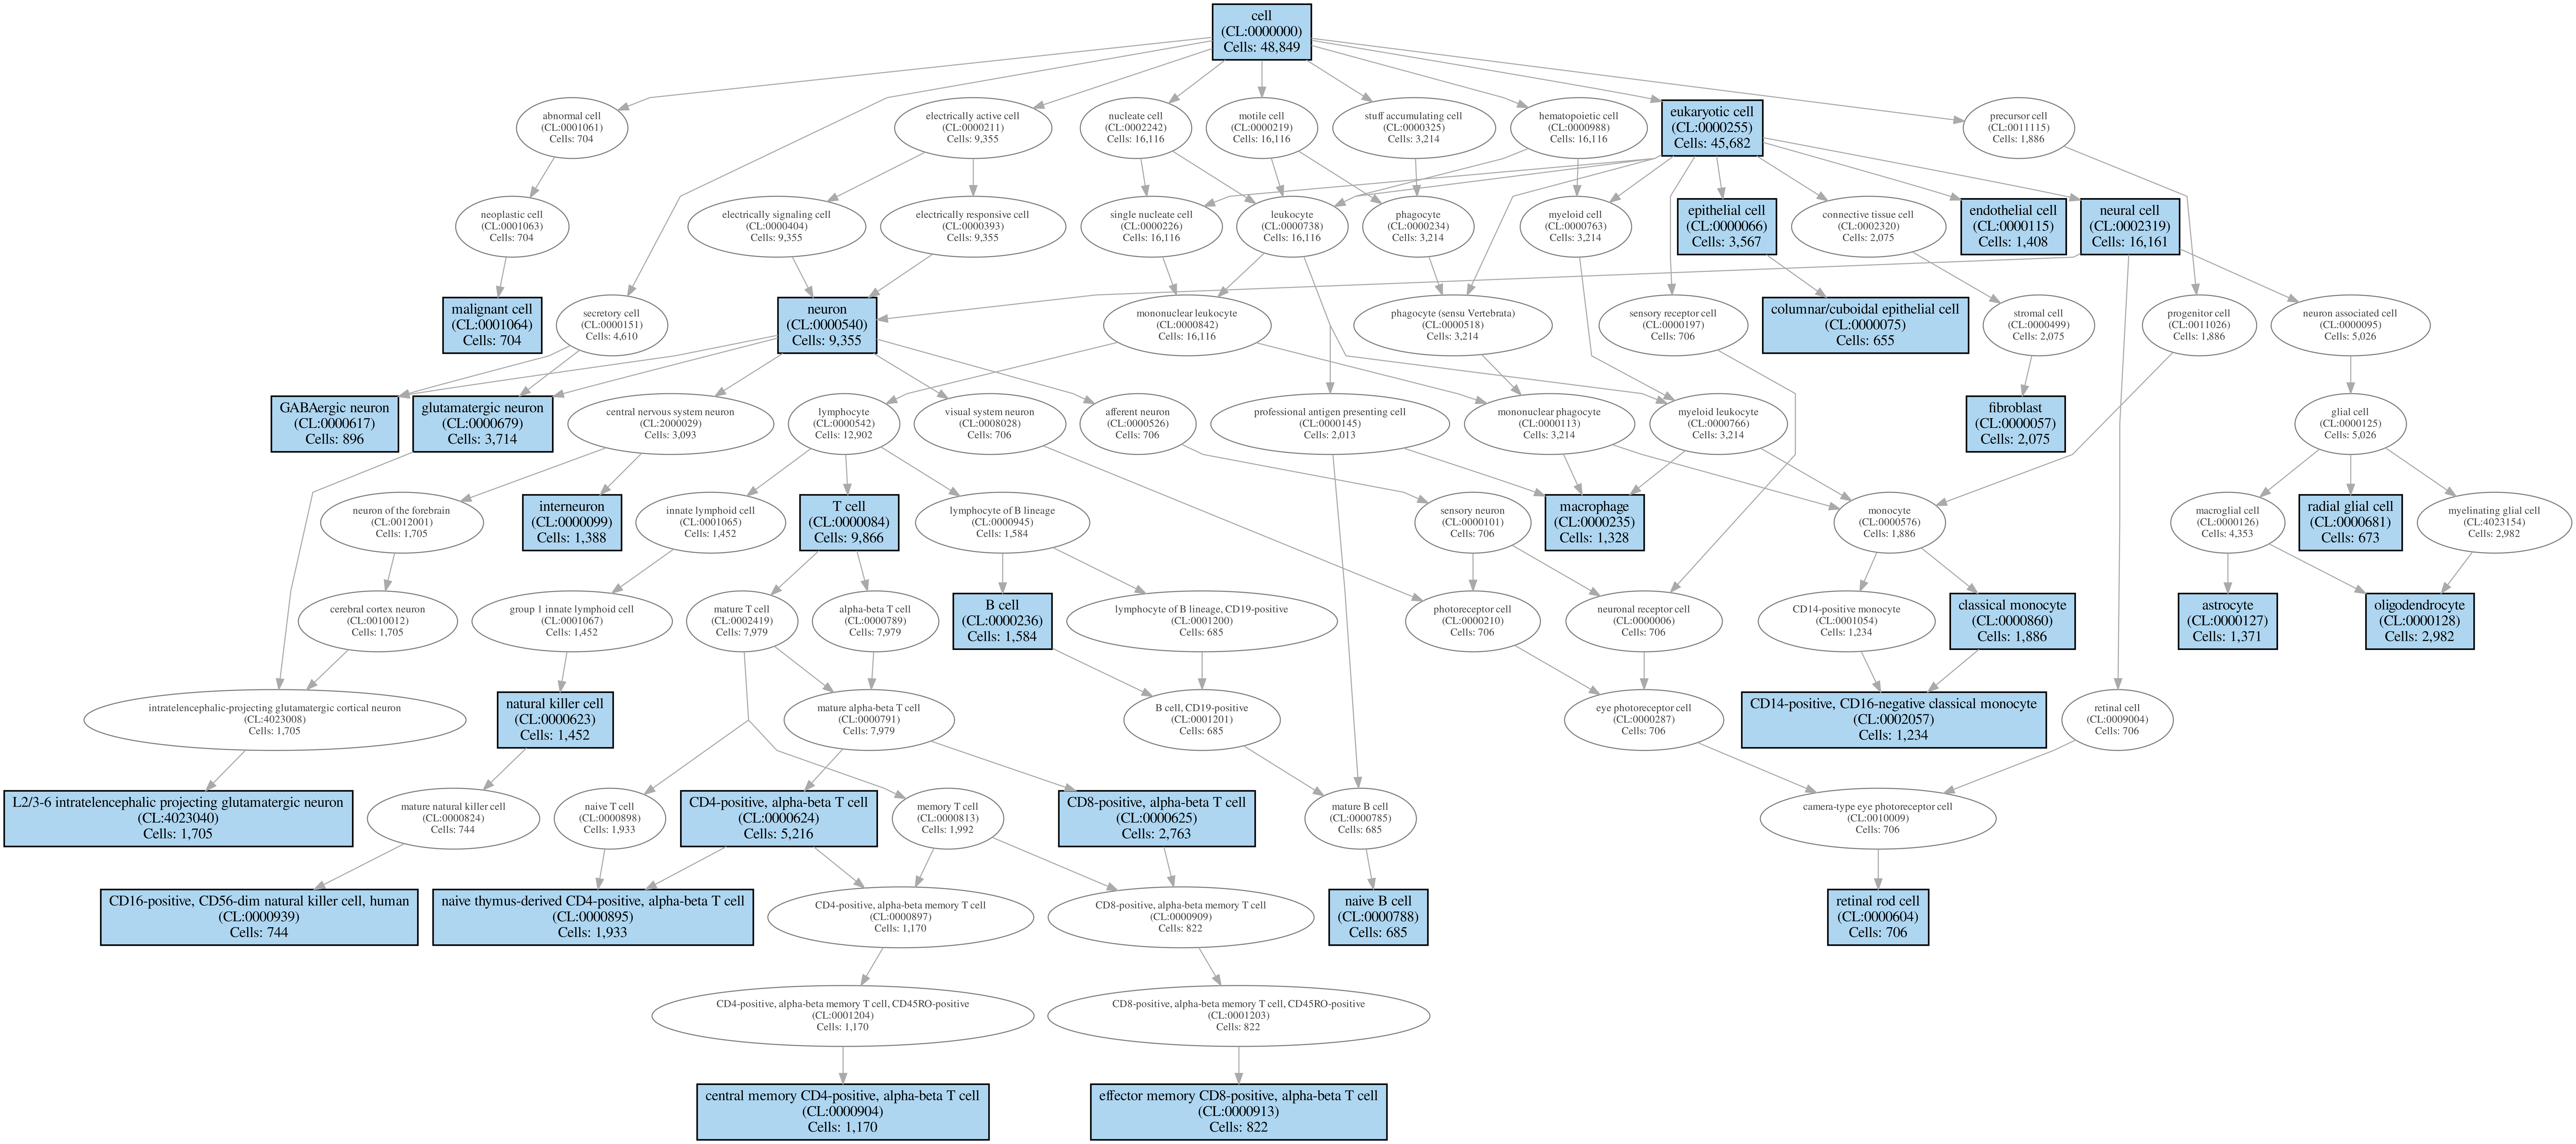
\includegraphics[width=\textwidth,height=0.78\textheight,keepaspectratio]{figures/supp_coarse_ontology_pruned.png}
\caption{Pruned Cell Ontology structure associated with the retained coarse-label anchors. The complete observed ontology is substantially wider and is distributed separately as searchable vector SVG and PDF files together with the exact fine-to-coarse mapping.}
\label{fig:supp-ontology}
\end{figure}

\FloatBarrier
\section{Experimental grids and shared training settings}
\label{sec:supp-grids}

Table~\ref{tab:supp-grids} summarises the four experimental grids.
Target parameter counts were converted into realised widths in multiples of four while retaining four attention heads.
The context/model-size sweep compares configurations after a common optimiser step within each formulation, whereas the learning-rate and architectural-shape sweeps compare configurations at matched estimated training FLOPs.

\begin{table}[ht]
\centering
\caption{Summary of the experimental grids.}
\label{tab:supp-grids}
\footnotesize
\resizebox{\textwidth}{!}{%
\begin{tabular}{p{0.19\textwidth}p{0.25\textwidth}p{0.28\textwidth}p{0.21\textwidth}}
\toprule
Experiment & Varied quantities & Fixed or derived quantities & Scale \\
\midrule
Batch-size selection & Batch size 4, 16, 32, 64, or 128; width 128, 256, 512, or 1,024 & Context 256; depth 6; learning rate $3\times10^{-4}$; one-cycle schedule; 15,000 steps & 20 configurations per formulation \\
Context and parameter count & Context 128, 256, 512, 1,024, or 2,048; width 128, 256, 512, or 768; depth 2--6 & Batch size 32; maximum learning rate $10^{-3}$; one-cycle schedule; at most 50,000 steps & 100 configurations per formulation \\
Learning-rate sweep & Target $N=10^6$, $10^7$, $10^8$, or $10^9$; depth 2, 6, or 20; five learning rates from $10^{-5}$ to $10^{-3}$ & Width selected in multiples of four; eight compute slices; warm-up then constant learning rate & 60 configurations per formulation \\
Depth/width sweep & Target $N=1$, 3, 10, 30, 100, 300, or 1,000 million; depth 2, 4, 8, 16, 24, 32, or 64 & Width matched to target size; learning rate predicted by the joint rule; seven compute slices & 49 configurations per formulation \\
\bottomrule
\end{tabular}%
}
\end{table}

\begin{table}[ht]
\centering
\caption{Training and evaluation constants shared by the principal sweeps unless stated otherwise.}
\label{tab:supp-training-constants}
\small
\begin{tabular}{p{0.27\textwidth}p{0.65\textwidth}}
\toprule
Item & Setting \\
\midrule
Optimizer & AdamW initialised with $\beta_1=0.9$, $\beta_2=0.95$, $\epsilon=10^{-8}$, and weight decay 0.01; one-cycle runs vary $\beta_1$ as described in Methods \\
Learning-rate warm-up & 500 steps from $10^{-6}$ times the target value in compute-matched sweeps \\
Gradient clipping & Global norm clipped to 1 \\
Precision & bfloat16 mixed precision \\
Batch size & 32 cells, physical and effective \\
Gradient accumulation & None \\
Attention heads & 4 \\
Feed-forward width & $4W$ \\
Activation and dropout & ReLU; dropout 0.2 at the locations described in Methods \\
Masking probability & 0.15 per eligible selected position \\
Validation cadence & Before the first update and every 500 optimiser steps in the context/model-size sweep; compute-matched sweeps use their configured validation intervals \\
Embedding aggregation & Mean over token-level encoder outputs \\
\bottomrule
\end{tabular}
\end{table}

The preliminary batch-size experiment motivated batch size 32 as an engineering compromise between memory requirements and cells processed per update.
It should not be interpreted as a universal optimum because comparisons at fixed optimiser step also change the number of cells processed and the training compute.

The compute-matched sweeps used a linear warm-up followed by a constant learning rate so that a loss read at an intermediate FLOP slice corresponds to a prefix of the same optimisation schedule, independent of the eventual stopping budget.
This interpretation would not hold for the one-cycle schedule used in the preliminary and context-length sweeps: its learning rate at a given step is defined relative to the requested total number of steps and therefore changes when that endpoint changes.

\section{Additional context-length and parameter-scaling diagnostics}
\label{sec:supp-context}

The full training trajectories reveal optimisation transients and incomplete runs that are hidden by terminal-loss summaries (Figure~\ref{fig:supp-training-curves}).
The ranked formulation develops a progressively stronger size dependence as context length increases.
The binned formulation shows a smaller terminal separation between model sizes and a greater contribution from run-to-run dispersion.
At contexts 128, 256, 512, 1,024, and 2,048, the largest ranked model's observed loss exceeds its held-out power-law prediction by 0.45\%, 2.40\%, 4.62\%, 5.60\%, and 7.15\%, respectively.
The corresponding signed binned differences are 17.41\%, 8.04\%, 0.69\%, $-2.02$\%, and 1.89\%, calculated as $(L_{\mathrm{observed}}-L_{\mathrm{predicted}})/L_{\mathrm{predicted}}$.
These single-architecture extrapolation checks support interpreting the fits as local empirical summaries rather than asymptotic loss laws.

\begin{figure}[p]
\centering
\begin{minipage}[t]{0.49\textwidth}
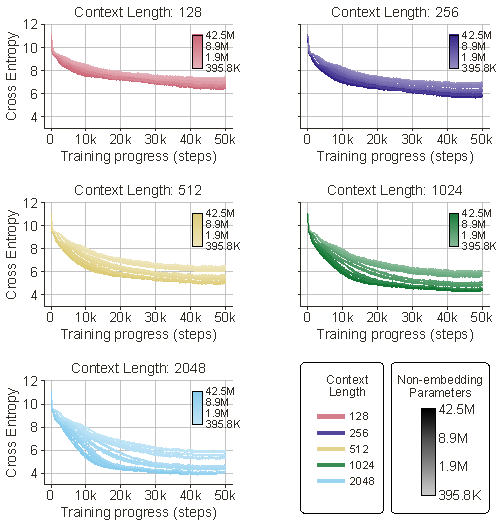
\includegraphics[width=\linewidth]{figures/supp_ranked_training_steps.pdf}
\end{minipage}\hfill
\begin{minipage}[t]{0.49\textwidth}
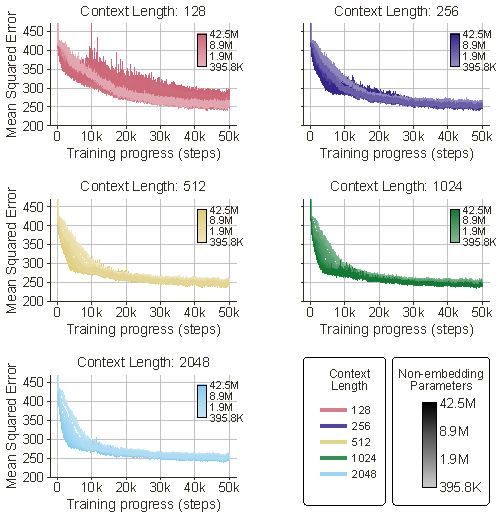
\includegraphics[width=\linewidth]{figures/supp_binned_training_steps.pdf}
\end{minipage}
\caption{Training-loss trajectories across context lengths and encoder architectures. Left, \ranked. Right, \binned. The binned loss is expression MSE on masked positions predicted active by the activity head, rather than the summed optimisation objective.}
\label{fig:supp-training-curves}
\end{figure}

Viewing the same fixed-step sweep against cumulative FLOPs is a useful diagnostic, but it is not a compute-optimal frontier: larger encoders consume more FLOPs at every optimiser step and therefore traverse the horizontal axis faster.
The FLOP values were obtained from an operator-level meta-device execution of the complete model forward pass and multiplied by three to approximate training, rather than from only the leading transformer term.
They therefore reflect differences among the instantiated architectures more directly than a leading-term estimate, but remain algorithmic estimates rather than measurements of accelerator time, utilisation, data loading, or optimiser overhead.

The principal scaling variable is the trainable non-embedding parameter count rather than the total parameter count.
With a vocabulary of 61,497 genes, the input embeddings and task-specific decoders can contribute many parameters whose scaling with width and functional role differ from those of the shared transformer encoder.
Using total parameters would therefore mix changes in encoder capacity with formulation-specific input and output modules, particularly when comparing architectural shapes; total counts remain useful accounting quantities but are not the independent size variable in the fitted scaling laws.

\begin{figure}[p]
\centering
\begin{minipage}[t]{0.49\textwidth}
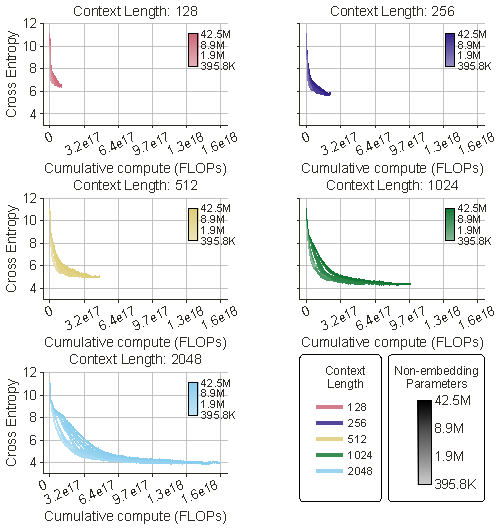
\includegraphics[width=\linewidth]{figures/supp_ranked_training_flops.pdf}
\end{minipage}\hfill
\begin{minipage}[t]{0.49\textwidth}
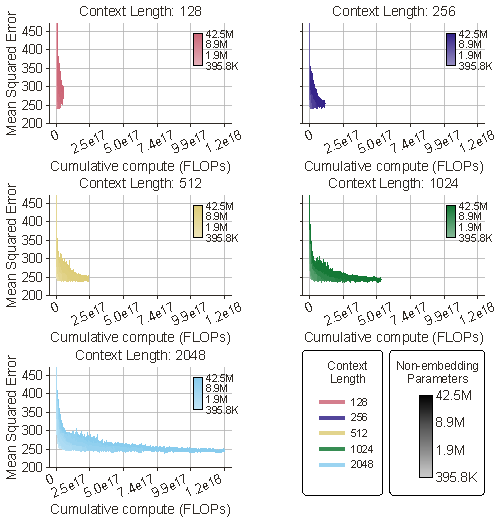
\includegraphics[width=\linewidth]{figures/supp_binned_training_flops.pdf}
\end{minipage}
\caption{Training loss as a function of cumulative estimated training FLOPs. Left, \ranked. Right, \binned. These trajectories arise from a fixed-step experiment and should not be read as an isoFLOP architecture comparison.}
\label{fig:supp-training-flops}
\end{figure}

\FloatBarrier
\section{Detailed downstream representation analyses}
\label{sec:supp-downstream}

\subsection{Metrics and terminal summaries}

BIOscore is the unweighted mean of nine biological-preservation and probe metrics: fine and coarse NMI, ARI, and homogeneity; label ASW; graph connectivity; and coarse-label ridge validation accuracy.
All are oriented so that larger values indicate better performance.
Batch ASW is reported separately because it measures source-dataset mixing rather than biological preservation and is not a BIOscore component.
The source-dataset identifier is also a much coarser grouping than a conventional experimental batch: source datasets may differ in donor composition, tissue sampling, protocol, laboratory, study design, and other biological or technical factors, rather than representing replicate samples generated under otherwise matched conditions.
It therefore cannot isolate a technical batch effect in the usual sense and is better interpreted as a descriptive measure of cross-dataset mixing.
No batch-correction procedure was applied, so this diagnostic characterises source-dataset structure already present in the learned embeddings and is given less interpretive weight than the biological-preservation metrics.

Two related but distinct clustering evaluations were performed at each checkpoint.
The components entering BIOscore used a fixed procedure: embeddings were projected to 50 principal components, a 15-nearest-neighbour graph was constructed with Euclidean distance, and Leiden clustering was run at resolution 1.0.
Fine-label metrics used all 30,000 validation cells; the graph and clustering were recomputed for the 29,252 cells with valid ontology-reduced labels before calculating coarse-label metrics.
Separately, the scIB evaluation operated on the raw mean-pooled embeddings and selected a Leiden resolution by maximising fine-label NMI over the ten values \(0.2, 0.4, \ldots, 2.0\).
The NMI and ARI from this resolution-optimised clustering were retained as scIB diagnostics but did not enter BIOscore.
Their purpose was a sensitivity check: if their trends had differed materially from the fixed-resolution results, this would have indicated that applying the same, label-independent clustering hyperparameter to every checkpoint unduly disadvantaged configurations with a different preferred cluster granularity.
They were excluded from BIOscore because they are alternative versions of NMI and ARI and would therefore count essentially the same clustering-agreement signal a second time.
Moreover, because the biological labels select the resolution, these values describe how well an embedding can support a favourable clustering over the searched resolutions; they are not label-free or held-out estimates of clustering performance and are expected to be somewhat optimistic relative to the fixed procedure.

For completeness, let \(U\) denote a clustering, \(Y\) the corresponding biological labels, \(n_{uy}\) their contingency-table counts, \(a_u=\sum_y n_{uy}\), \(b_y=\sum_u n_{uy}\), and \(n=\sum_{u,y}n_{uy}\).
The arithmetic normalisation of mutual information used here is
\begin{align}
I(U;Y) &= \sum_{u,y}\frac{n_{uy}}{n}
\log\!\left(\frac{n\,n_{uy}}{a_u b_y}\right), \\
\operatorname{NMI}(U,Y) &= \frac{2I(U;Y)}{H(U)+H(Y)},
\end{align}
with zero-count terms omitted.
NMI ranges from zero for partitions sharing no information to one for identical partitions, subject to the chosen normalisation.
ARI instead counts agreement over pairs of cells and corrects its expected value under random partitions:
\begin{equation}
\operatorname{ARI}
=\frac{
\displaystyle\sum_{u,y}\binom{n_{uy}}{2}
-\displaystyle\frac{\left[\sum_u\binom{a_u}{2}\right]
\left[\sum_y\binom{b_y}{2}\right]}{\binom{n}{2}}
}{
\displaystyle\frac{1}{2}\left[
\sum_u\binom{a_u}{2}+\sum_y\binom{b_y}{2}
\right]
-\displaystyle\frac{\left[\sum_u\binom{a_u}{2}\right]
\left[\sum_y\binom{b_y}{2}\right]}{\binom{n}{2}}
}.
\end{equation}
An ARI of one denotes identical partitions, zero is the random-partition baseline, and negative values indicate less agreement than that baseline.
Homogeneity is
\begin{equation}
h(Y,U)=1-\frac{H(Y\mid U)}{H(Y)},
\end{equation}
with the conventional value one when \(H(Y)=0\).
It asks whether each inferred cluster contains cells from only one biological label, but, unlike a completeness criterion, it does not by itself penalise splitting one label across many pure clusters.

For a cell \(i\), let \(a(i)\) be its mean distance to cells with the same label and let \(b(i)\) be the smallest mean distance to cells carrying any other label.
The raw silhouette coefficient is
\begin{equation}
s(i)=\frac{b(i)-a(i)}{\max\{a(i),b(i)\}}.
\end{equation}
The reported label ASW is \((1+\overline{s})/2\), so values near one indicate compact, well-separated biological labels and values near one half indicate substantial overlap.
Batch ASW reverses the objective after calculating source-dataset silhouettes within each eligible fine cell type:
\begin{equation}
\operatorname{ASW}_{\mathrm{batch}}
=\frac{1}{|\mathcal{C}_{\mathrm{elig}}|}
\sum_{c\in\mathcal{C}_{\mathrm{elig}}}
\frac{1}{|V_c|}\sum_{i\in V_c}\left(1-|s_{\mathrm{batch}}(i)|\right).
\end{equation}
Consequently, the scaled value reported here is larger when source datasets mix more thoroughly within a biological label.
Cell types containing only one represented dataset, or one dataset per cell, cannot define this quantity and were omitted by the implementation.

Graph connectivity measures whether each biological population remains connected in the neighbour graph:
\begin{equation}
\operatorname{GC}=\frac{1}{|\mathcal{C}|}
\sum_{c\in\mathcal{C}}
\frac{|\operatorname{LCC}(G_c)|}{|V_c|},
\end{equation}
where \(G_c\) is the graph induced by cells with label \(c\), \(V_c\) is its vertex set, and \(\operatorname{LCC}\) is its largest connected component.
This score is one when every cell type forms a connected subgraph, but it does not require different cell types to be separated from one another.
The ridge-probe metric is ordinary classification accuracy on the stratified 20\% probe-validation split; unlike the clustering scores, it evaluates linear decodability rather than unsupervised partition agreement.

\begin{table}[ht]
\centering
\caption{Downstream metric definitions and their use in BIOscore.}
\label{tab:supp-metric-definitions}
\small
\begin{tabular}{p{0.21\textwidth}p{0.62\textwidth}p{0.09\textwidth}}
\toprule
Metric & Interpretation & BIOscore \\
\midrule
Fine/coarse NMI & Mutual information between fixed-resolution Leiden clusters and fine or ontology-reduced cell types, normalised for partition entropy & Yes \\
Fine/coarse ARI & Pairwise agreement between the same cluster assignments and labels, adjusted for chance & Yes \\
Fine/coarse homogeneity & Degree to which each cluster contains cells from a single fine or coarse label & Yes \\
Label ASW & Silhouette separation by fine biological label, linearly scaled to $[0,1]$ & Yes \\
Graph connectivity & Mean fraction of each fine cell type retained in its largest connected component & Yes \\
Coarse ridge accuracy & Validation accuracy of the unstandardised, no-intercept ridge probe on coarse labels & Yes \\
Resolution-optimised NMI/ARI & Sensitivity check after selecting the Leiden resolution that maximises fine-label NMI; excluded to avoid duplicating fixed-resolution NMI/ARI & No \\
Batch ASW & Within-cell-type mixing of source datasets; a coarse source-domain diagnostic rather than a controlled replicate batch-effect measure & No \\
\bottomrule
\end{tabular}
\end{table}

Writing \(\mathcal{Q}\) for the available BIOscore components in a checkpoint row, the composite is
\begin{equation}
\operatorname{BIOscore}=\frac{1}{|\mathcal{Q}|}\sum_{q\in\mathcal{Q}}q.
\end{equation}
This is a study-specific visual summary rather than a standard scIB score or a calibrated measure of biological utility.
Six of its nine terms are derived from the two fixed-resolution Leiden partitions, so the unweighted average gives clustering agreement substantial numerical influence; the component plots and tables should therefore remain the primary basis for interpretation.
The constituent scores also have different null behaviour---most lie in \([0,1]\), whereas ARI is chance-adjusted and may be negative---and correlated components should not be read as nine independent confirmations of a trend.

Table~\ref{tab:supp-terminal-downstream} reports means over the terminal checkpoint of all architectures at each context length.
For the ranked formulation, mean terminal BIOscore rises from 0.232 at context 128 to 0.353 at context 1,024 and then falls to 0.323 at context 2,048.
For the binned formulation it rises from 0.176 to 0.345 across the tested context range.
The corresponding mean terminal-minus-initial changes are $+0.173$ and $+0.150$, respectively, when averaged over runs.
These descriptive averages summarise the grid and do not supply repeated-seed uncertainty.

\begin{table}[p]
\centering
\caption{Mean terminal downstream metrics by formulation and context length. Each mean summarises 20 architectures, with one training run per architecture and one terminal checkpoint per run; these are not independent seed replicates. f/c denote fine/coarse labels; Hom, homogeneity; LASW, label ASW; GC, graph connectivity; Ridge, coarse ridge validation accuracy; BASW, source-dataset ASW. BASW is a coarse cross-dataset mixing diagnostic, not a controlled replicate batch-effect measure, and is not included in BIOscore.}
\label{tab:supp-terminal-downstream}
\scriptsize
\resizebox{\textwidth}{!}{%
\begin{tabular}{llrrrrrrrrrrr}
\toprule
Formulation & Context & BIO & fNMI & fARI & fHom & cNMI & cARI & cHom & LASW & GC & Ridge & BASW \\
\midrule
Ranked & 128   & .232 & .279 & .071 & .213 & .254 & .087 & .228 & .340 & .359 & .258 & .841 \\
Ranked & 256   & .284 & .357 & .101 & .279 & .341 & .129 & .318 & .331 & .405 & .295 & .814 \\
Ranked & 512   & .341 & .429 & .174 & .344 & .420 & .195 & .404 & .305 & .450 & .344 & .772 \\
Ranked & 1,024 & .353 & .450 & .191 & .373 & .436 & .201 & .438 & .242 & .461 & .385 & .695 \\
Ranked & 2,048 & .323 & .415 & .151 & .356 & .391 & .155 & .407 & .181 & .439 & .411 & .632 \\
\midrule
Binned & 128   & .176 & .215 & .049 & .165 & .181 & .059 & .164 & .221 & .323 & .210 & .731 \\
Binned & 256   & .260 & .328 & .119 & .255 & .311 & .138 & .287 & .248 & .366 & .290 & .727 \\
Binned & 512   & .309 & .390 & .160 & .311 & .379 & .168 & .359 & .264 & .412 & .338 & .727 \\
Binned & 1,024 & .341 & .429 & .171 & .349 & .419 & .192 & .408 & .259 & .450 & .391 & .709 \\
Binned & 2,048 & .345 & .438 & .168 & .365 & .421 & .180 & .423 & .225 & .472 & .410 & .674 \\
\bottomrule
\end{tabular}%
}
\end{table}

\begin{table}[ht]
\centering
\caption{Mean terminal resolution-optimised scIB clustering metrics by formulation and context length. Each mean summarises 20 architectures, with one training run per architecture and one terminal checkpoint per run. These diagnostics use fine labels, and neither enters BIOscore.}
\label{tab:supp-terminal-scib-clustering}
\small
\begin{tabular}{lrrr}
\toprule
Formulation & Context & Optimised NMI & Optimised ARI \\
\midrule
Ranked & 128   & .295 & .076 \\
Ranked & 256   & .371 & .108 \\
Ranked & 512   & .440 & .175 \\
Ranked & 1,024 & .460 & .180 \\
Ranked & 2,048 & .434 & .146 \\
\midrule
Binned & 128   & .228 & .051 \\
Binned & 256   & .338 & .125 \\
Binned & 512   & .402 & .153 \\
Binned & 1,024 & .447 & .180 \\
Binned & 2,048 & .459 & .178 \\
\bottomrule
\end{tabular}
\end{table}

The clustering metrics show the clearest and most internally concordant training trends.
Both fine- and coarse-label NMI, ARI, and homogeneity rise rapidly during early training and generally continue improving more slowly thereafter (Figures~\ref{fig:supp-ranked-fine}--\ref{fig:supp-binned-coarse}).
Longer context is beneficial up to 1,024 genes for the ranked formulation; at context 2,048, several ranked clustering curves plateau below the context-1,024 curves.
The binned formulation exhibits a more monotonic context trend, although fine and coarse ARI saturate between contexts 1,024 and 2,048.
The resolution-optimised scIB NMI and ARI show the same broad context-length trends (Table~\ref{tab:supp-terminal-scib-clustering} and Figures~\ref{fig:supp-ranked-batch} and~\ref{fig:supp-binned-batch}).
This agreement supports the robustness of the broad context-length trends to the clustering-resolution choice; it does not establish that every configuration is equally well served by the fixed resolution.
They were not added to BIOscore because doing so would redundantly count NMI and ARI twice, while optimisation against fine-label NMI also makes the resolution-optimised versions less conservative summaries.

Graph connectivity and coarse ridge accuracy also improve with context and training, but they do not duplicate the clustering metrics (Figures~\ref{fig:supp-ranked-representation} and~\ref{fig:supp-binned-representation}).
In particular, terminal ridge accuracy is dominated by context length and is not consistently monotonic with non-embedding parameter count within a fixed context.
Its interpretation is further limited by the increase in embedding dimensionality with model width.

Label ASW and source-dataset ASW expose a useful descriptive tension that is hidden by BIOscore.
At longer contexts, biological clustering and graph connectivity improve while terminal source-dataset ASW decreases in both formulations (Figures~\ref{fig:supp-ranked-batch} and~\ref{fig:supp-binned-batch}).
Thus improved clustering agreement and connectivity do not imply increasing cross-dataset mixing or improved silhouette separation in these uncorrected embeddings.
However, because dataset of origin conflates potentially large biological and technical differences and does not represent matched experimental replicates, this trend should not be interpreted as evidence about conventional batch correction and is less relevant to model quality than the biological-label metrics.

\begin{figure}[p]
\centering
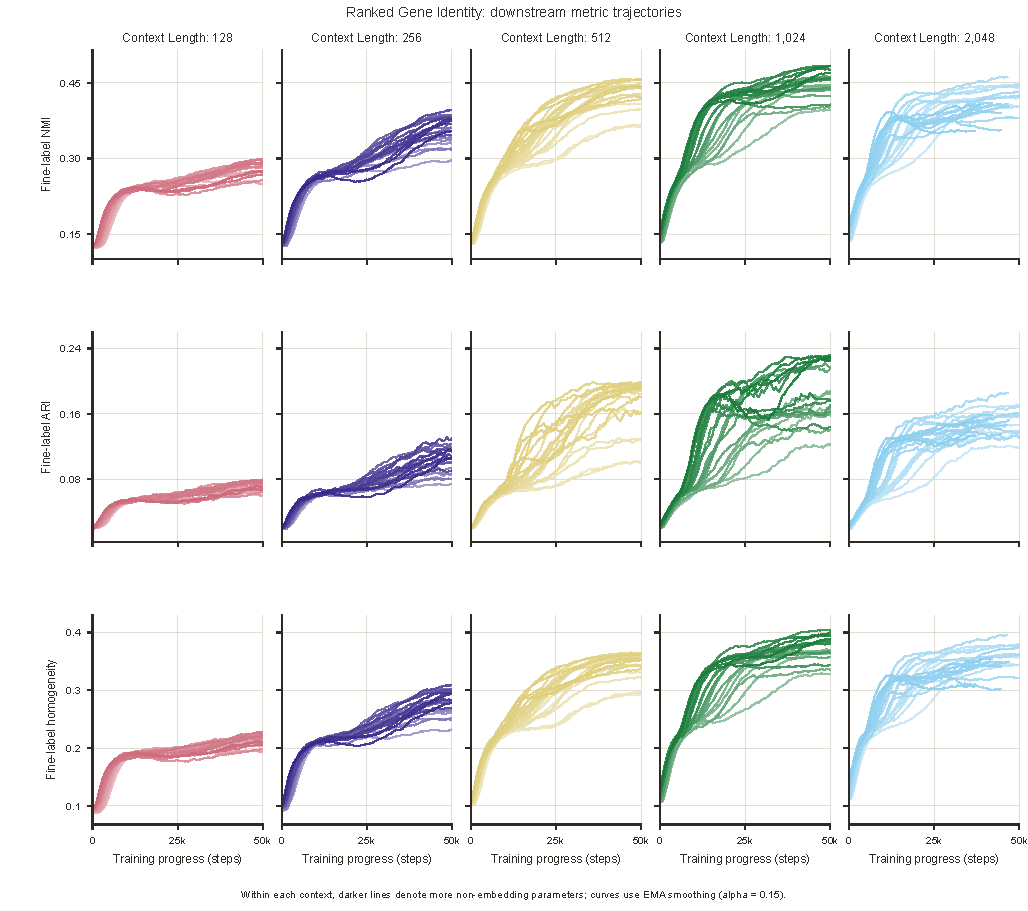
\includegraphics[width=\textwidth]{figures/supp_ranked_downstream_fine.pdf}
\caption{Fine-label clustering trajectories for the \ranked\ formulation. Each column is a context length and each row is one BIOscore component. Within a panel, darker curves denote more non-embedding parameters.}
\label{fig:supp-ranked-fine}
\end{figure}

\begin{figure}[p]
\centering
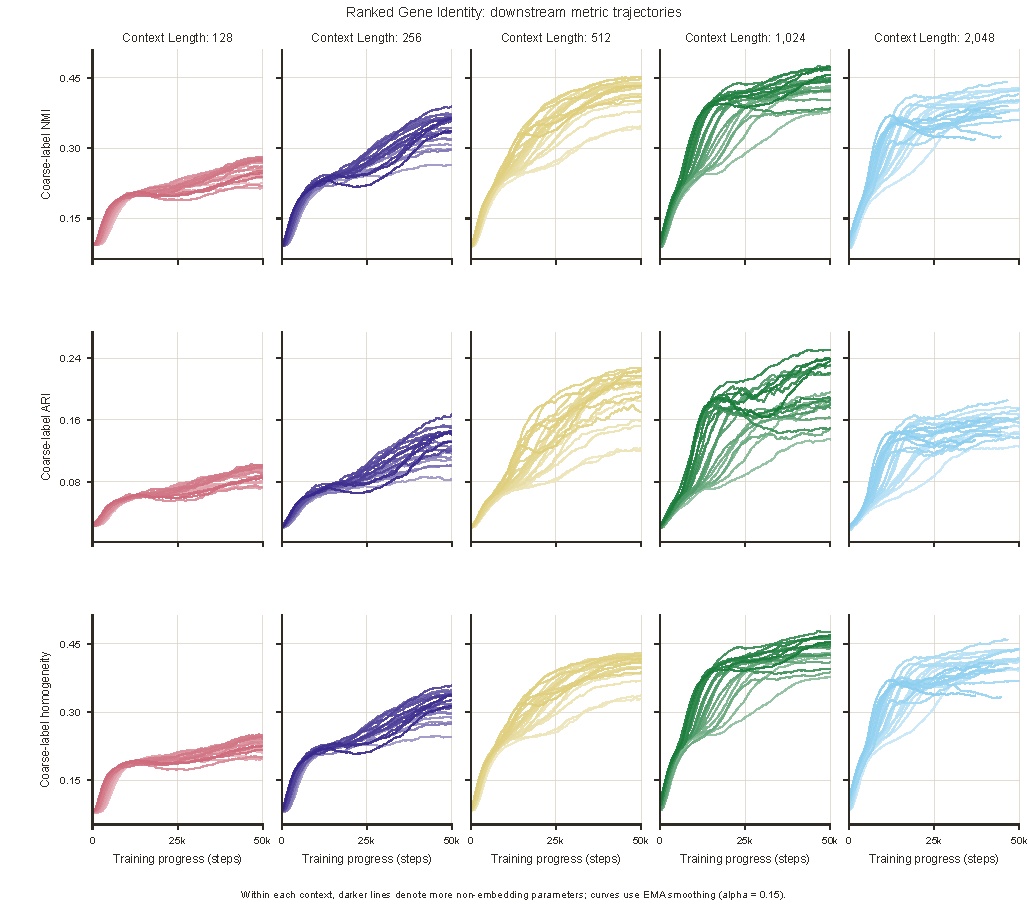
\includegraphics[width=\textwidth]{figures/supp_ranked_downstream_coarse.pdf}
\caption{Coarse-label clustering trajectories for the \ranked\ formulation. Coarse metrics exclude cells assigned the special label \texttt{unknown}.}
\label{fig:supp-ranked-coarse}
\end{figure}

\begin{figure}[p]
\centering
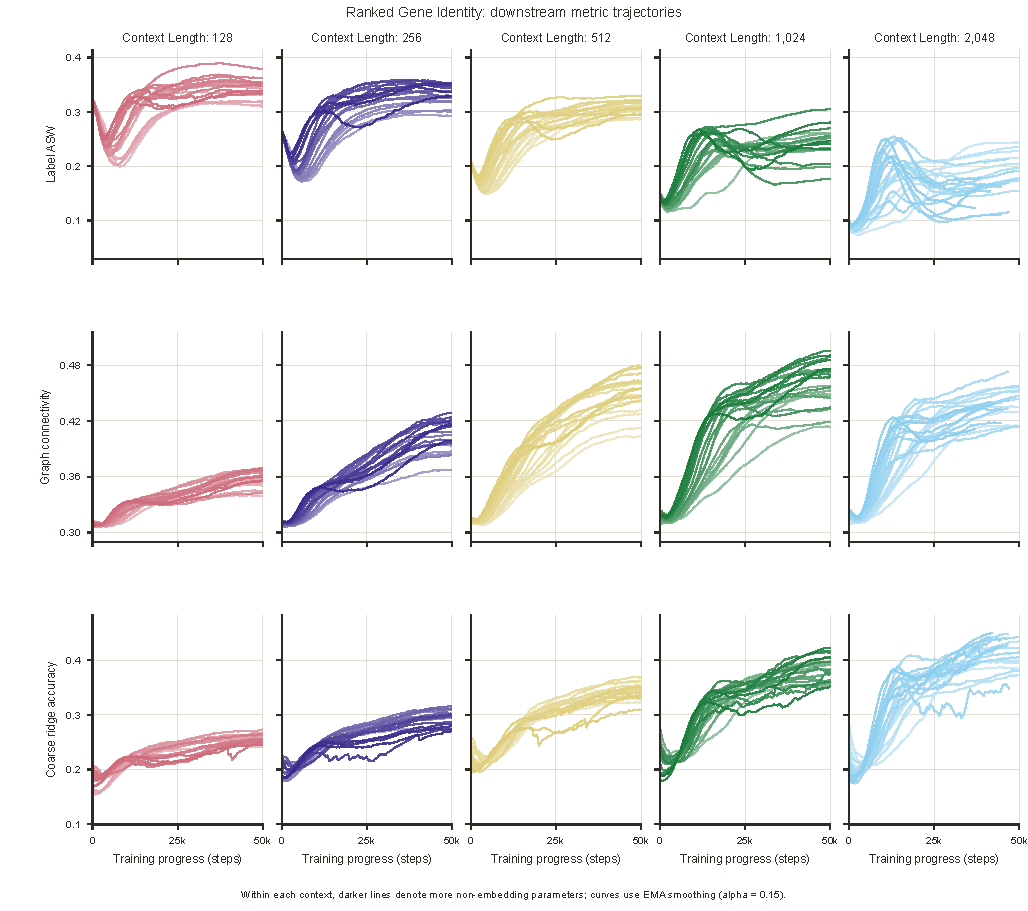
\includegraphics[width=\textwidth]{figures/supp_ranked_downstream_representation.pdf}
\caption{Label ASW, graph connectivity, and coarse ridge-probe accuracy for the \ranked\ formulation. These three metrics enter BIOscore but capture distinct aspects of the embedding geometry.}
\label{fig:supp-ranked-representation}
\end{figure}

\begin{figure}[p]
\centering
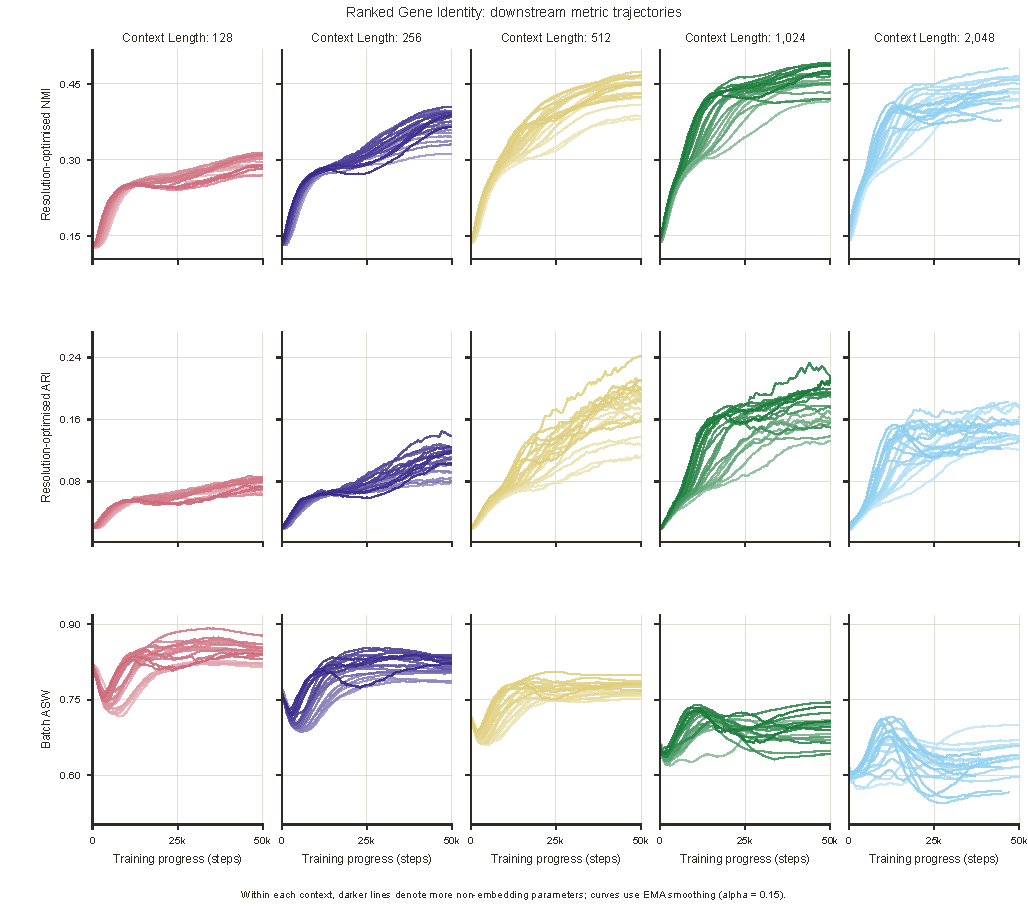
\includegraphics[width=\textwidth]{figures/supp_ranked_downstream_batch.pdf}
\caption{Resolution-optimised fine-label NMI and ARI together with source-dataset ASW for the \ranked\ formulation. At every checkpoint, the Leiden resolution was selected by maximising fine-label NMI over ten candidate values as a sensitivity check on the fixed-resolution comparison. Larger ASW values indicate greater source-dataset mixing within fine cell types; dataset of origin is a coarse source-domain label rather than a controlled replicate batch. None of these three scIB diagnostics enters BIOscore.}
\label{fig:supp-ranked-batch}
\end{figure}

\begin{figure}[p]
\centering
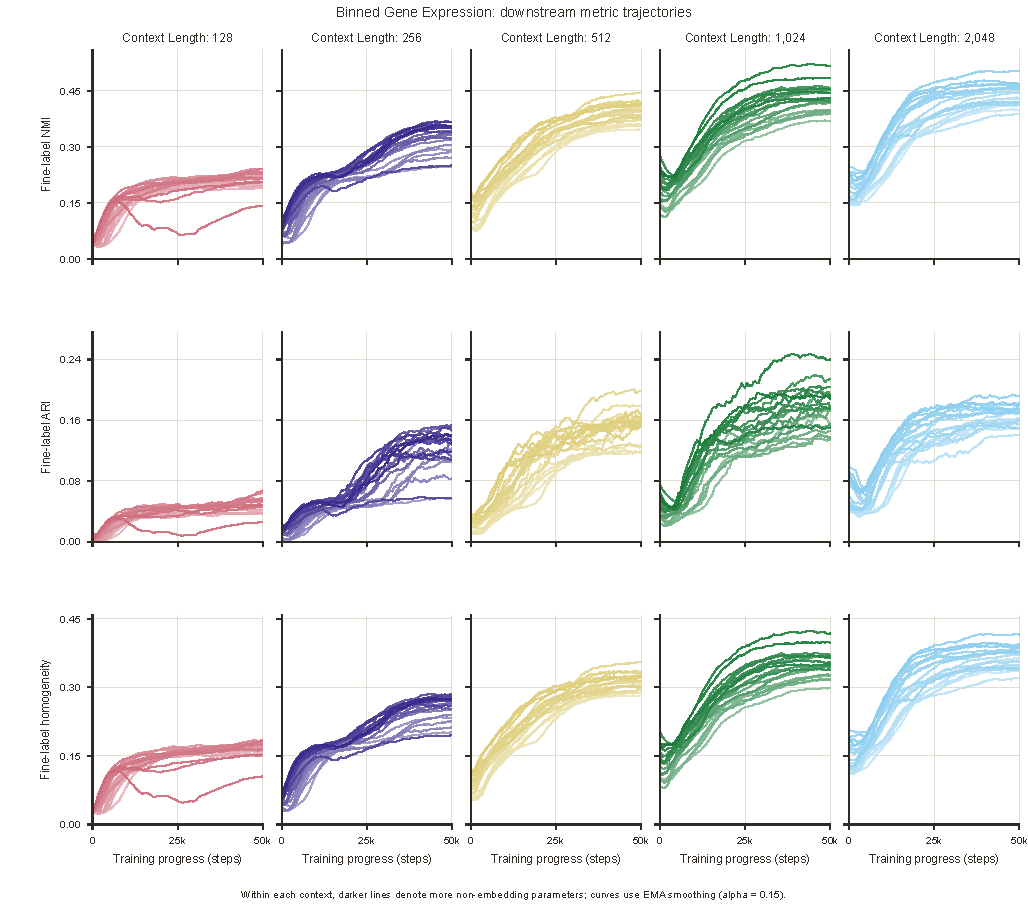
\includegraphics[width=\textwidth]{figures/supp_binned_downstream_fine.pdf}
\caption{Fine-label clustering trajectories for the \binned\ formulation. Plot encodings match Figure~\ref{fig:supp-ranked-fine}.}
\label{fig:supp-binned-fine}
\end{figure}

\begin{figure}[p]
\centering
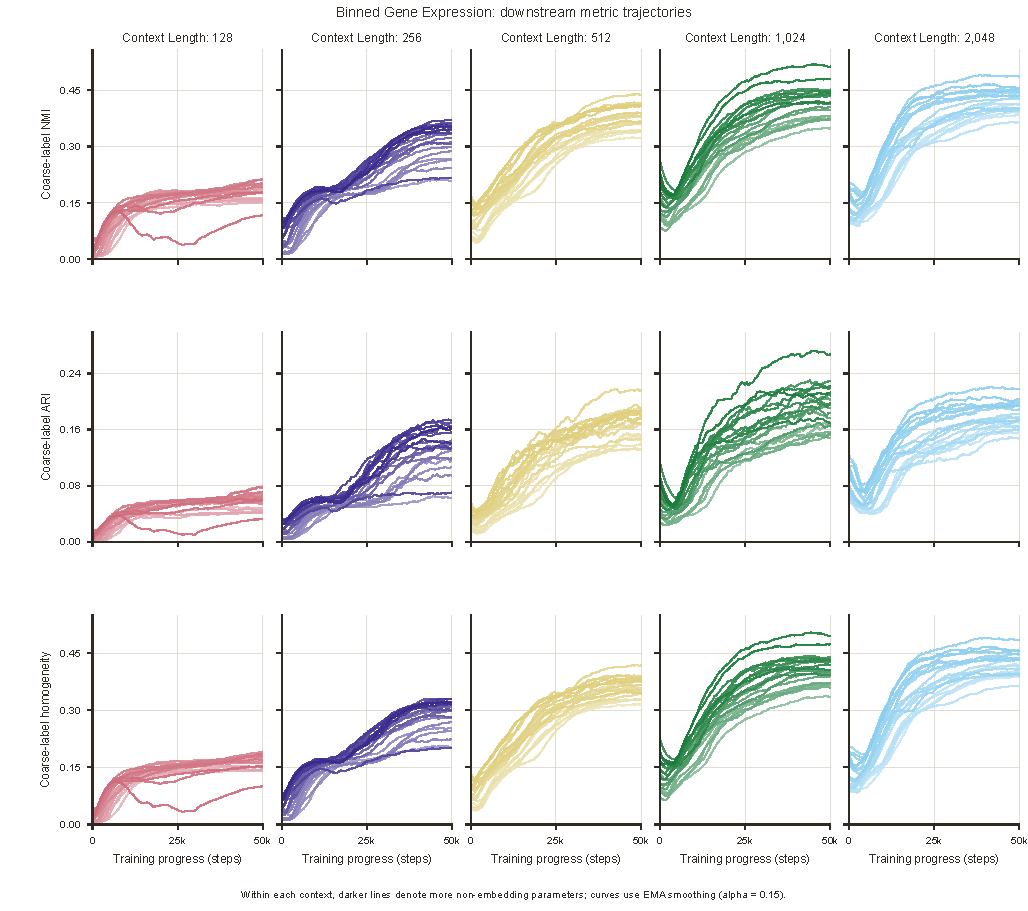
\includegraphics[width=\textwidth]{figures/supp_binned_downstream_coarse.pdf}
\caption{Coarse-label clustering trajectories for the \binned\ formulation.}
\label{fig:supp-binned-coarse}
\end{figure}

\begin{figure}[p]
\centering
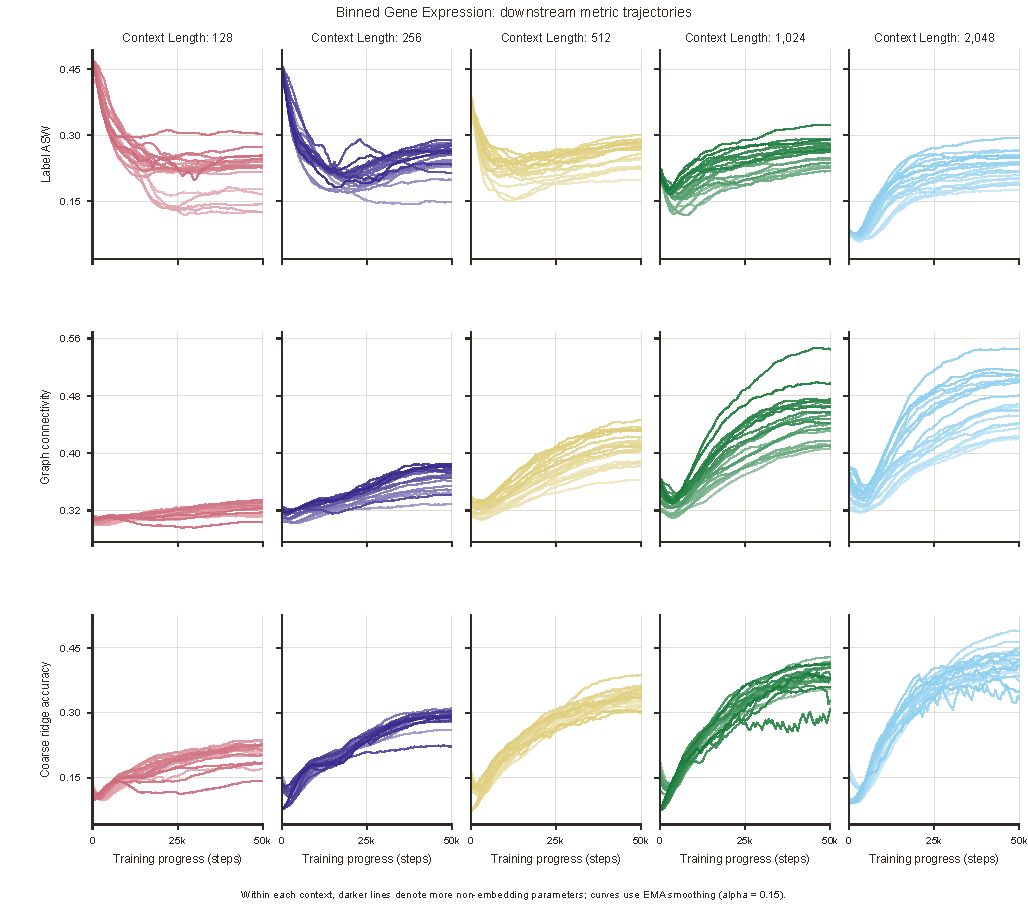
\includegraphics[width=\textwidth]{figures/supp_binned_downstream_representation.pdf}
\caption{Label ASW, graph connectivity, and coarse ridge-probe accuracy for the \binned\ formulation.}
\label{fig:supp-binned-representation}
\end{figure}

\begin{figure}[p]
\centering
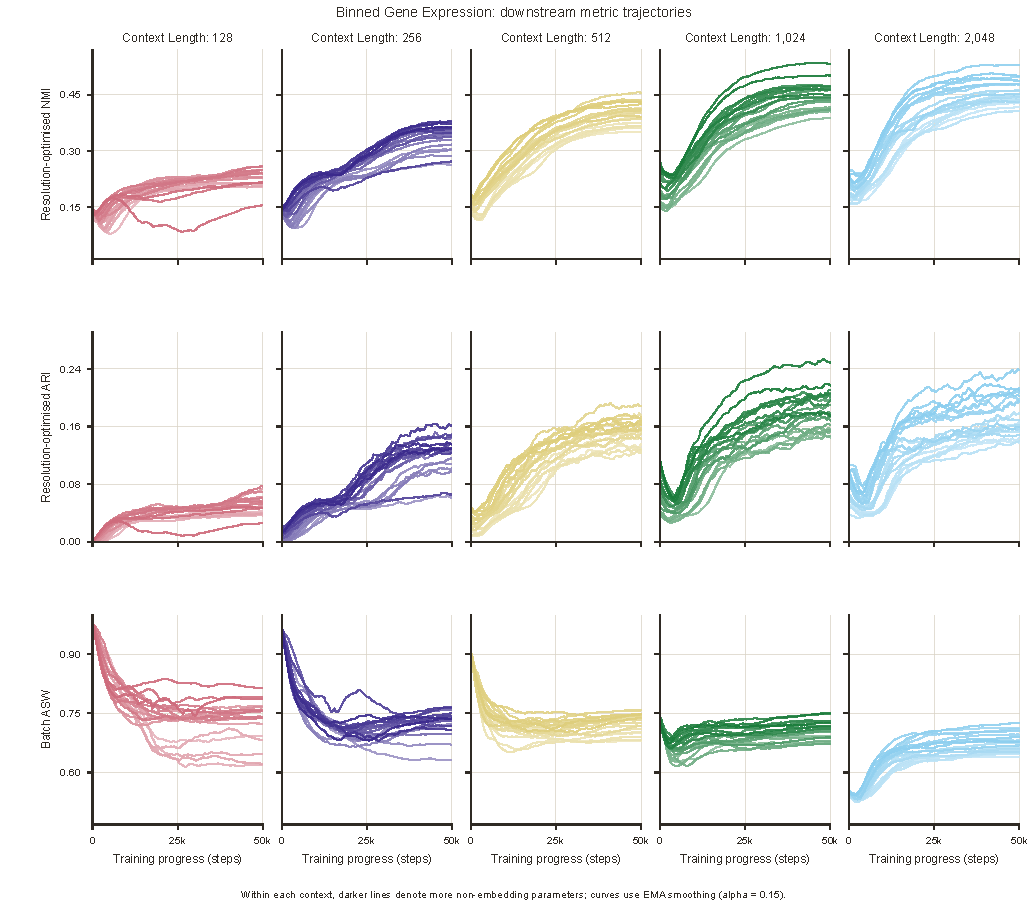
\includegraphics[width=\textwidth]{figures/supp_binned_downstream_batch.pdf}
\caption{Resolution-optimised fine-label NMI and ARI together with source-dataset ASW for the \binned\ formulation. Interpretation and exclusion criteria match Figure~\ref{fig:supp-ranked-batch}; none of these three scIB diagnostics enters BIOscore.}
\label{fig:supp-binned-batch}
\end{figure}

\FloatBarrier
\section{Learning-rate sweep diagnostics}
\label{sec:supp-learning-rate}

For each parameter/depth pair, the sampled learning rate with the smallest loss was identified at each compute slice.
When this discrete minimum had immediate neighbours on both sides in the original five-point learning-rate grid, and all three runs had finite losses and reached the completion threshold, a local quadratic was fitted in $\log_{10}\lambda$,
\begin{equation}
L=a_2[\log_{10}(\lambda)]^2+a_1\log_{10}(\lambda)+a_0.
\end{equation}
The continuous vertex was accepted only when $a_2>0$ and the vertex fell inside the three-point fitting interval.
All other cases retained the best eligible sampled optimum and should be read as discretised or potentially censored estimates. In particular, incomplete runs are not removed before defining adjacency: the estimator is not allowed to span across a missing or unfinished point to construct an artificial three-point window.

Figures~\ref{fig:supp-ranked-lr-sweeps} and~\ref{fig:supp-binned-lr-sweeps} overlay the accepted local quadratics and their inferred vertices at the last analysed compute slice (75\% of the target budget) used in the main figure.
Eleven of the twelve ranked architecture points admit an interior quadratic optimum, compared with seven of twelve binned points.
For the binned 1-million-parameter, depth-2 model, the immediate higher neighbour at $3\times10^{-4}$ reached only 10.0\% of its requested training duration. The guarded procedure therefore retains the best eligible sampled value, $10^{-4}$, rather than fitting a parabola through $3\times10^{-5}$, $10^{-4}$, and the non-adjacent $10^{-3}$ point.
Several binned curves are visibly shallow, particularly at the smaller parameter targets, so a numerically defined vertex can still be weakly localised even when it passes the acceptance rule.

\begin{figure}[p]
\centering
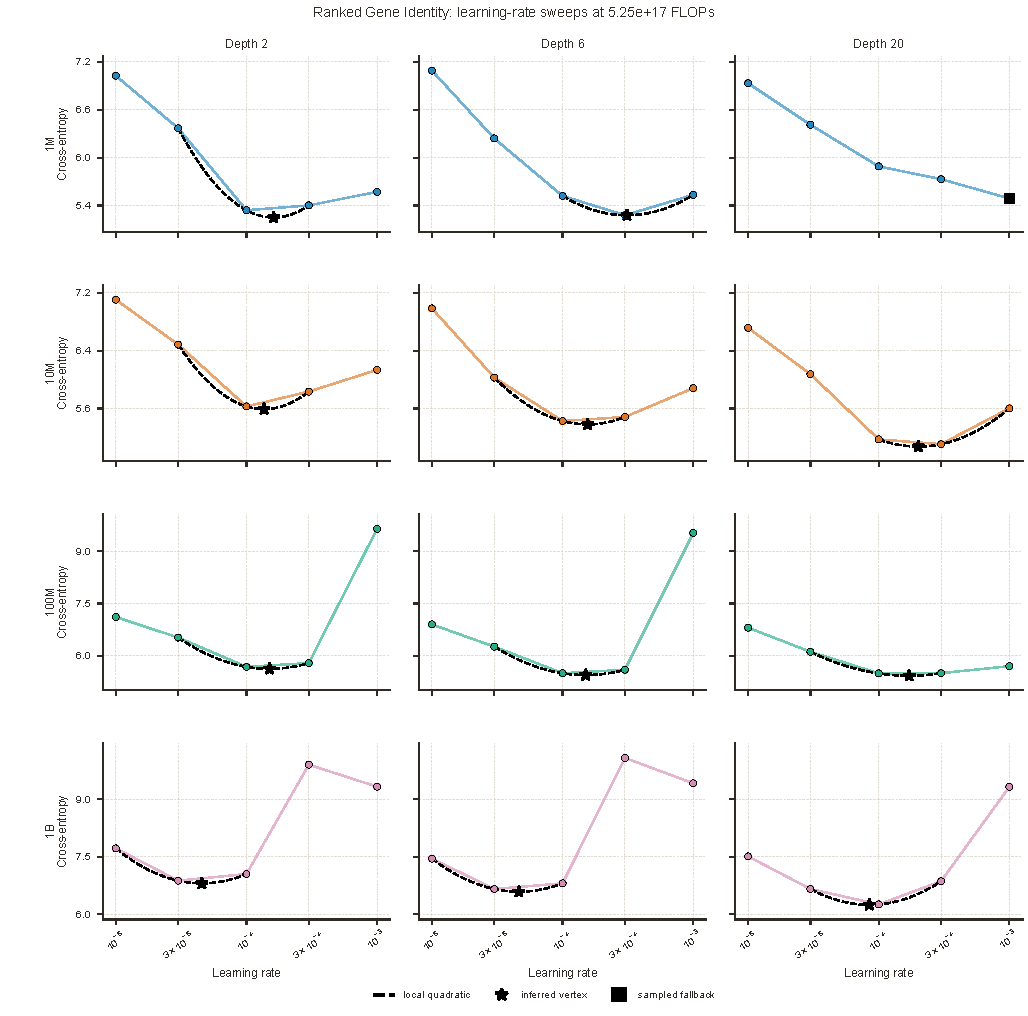
\includegraphics[width=\textwidth]{figures/supp_ranked_lr_sweeps.pdf}
\caption{\ranked\ learning-rate sweeps at $5.25\times10^{17}$ matched training FLOPs. Circles show eligible sampled runs, white circles show incomplete samples, dashed segments show accepted local quadratic fits, stars mark inferred vertices, and squares mark sampled fallbacks.}
\label{fig:supp-ranked-lr-sweeps}
\end{figure}

\begin{figure}[p]
\centering
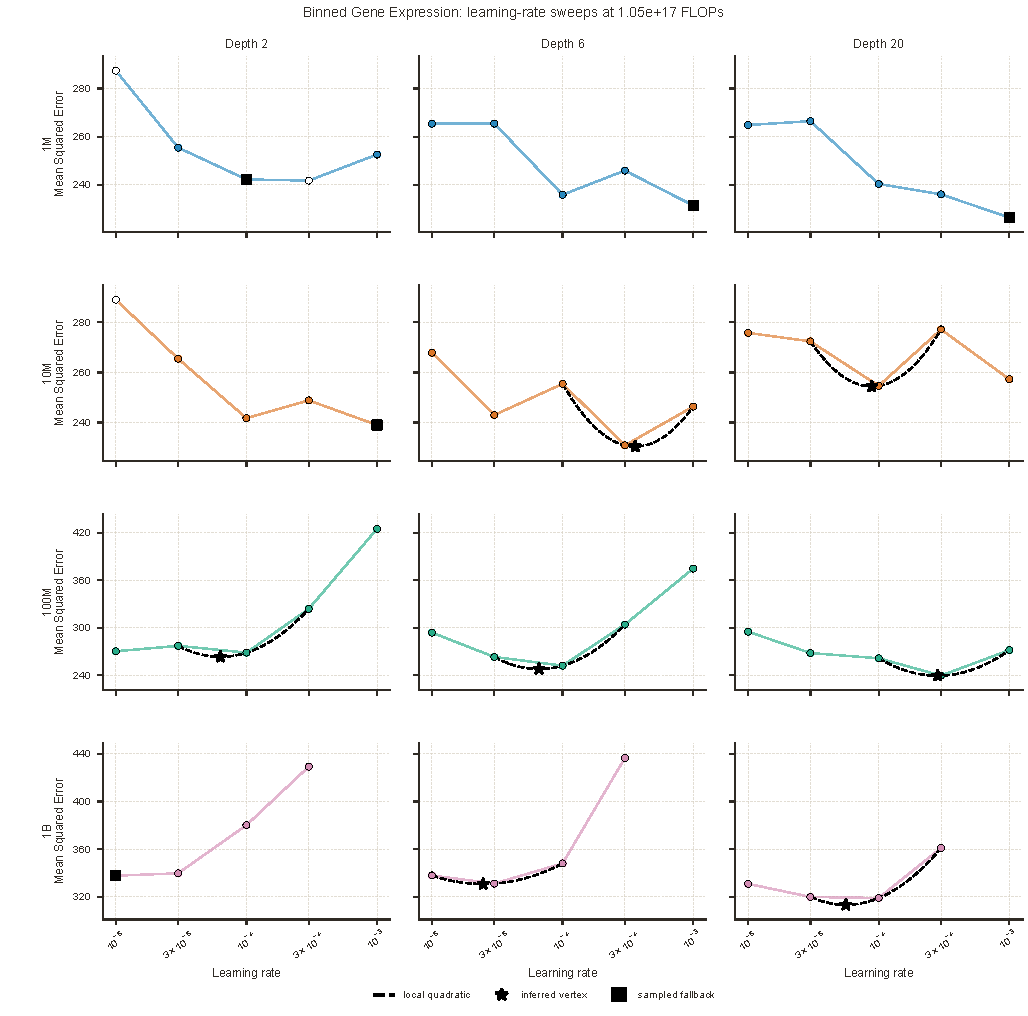
\includegraphics[width=\textwidth]{figures/supp_binned_lr_sweeps.pdf}
\caption{\binned\ learning-rate sweeps at $1.05\times10^{17}$ matched training FLOPs, with the same notation as Figure~\ref{fig:supp-ranked-lr-sweeps}. Non-finite or unavailable samples are omitted.}
\label{fig:supp-binned-lr-sweeps}
\end{figure}

The architecture-level optima were summarised with
\begin{equation}
\log_{10}\lambda^*=\beta_0+\alpha_N\log_{10}N+\alpha_D\log_{10}D.
\end{equation}
Across all eight compute slices, the size exponent is negative for both formulations (Table~\ref{tab:supp-lr-slices}).
The ranked depth exponent remains positive and its joint-model RMSE ranges from 0.086 to 0.150 dex.
The binned depth exponent is much less stable, ranging from $-0.175$ to $0.807$, and its RMSE ranges from 0.250 to 0.435 dex.
This variation is consistent with the shallower and less regular binned sweep profiles.

\begin{table}[p]
\centering
\caption{Joint learning-rate rule across matched-compute slices. $\alpha_N$ and $\alpha_D$ are the size and depth exponents; error is RMSE in $\log_{10}\lambda$ (dex); Q/F gives the number of accepted quadratic optima and sampled fallbacks among 12 architecture points.}
\label{tab:supp-lr-slices}
\scriptsize
\begin{tabular}{r rrrr rrrr}
\toprule
& \multicolumn{4}{c}{Ranked Gene Identity} & \multicolumn{4}{c}{Binned Gene Expression} \\
\cmidrule(lr){2-5}\cmidrule(lr){6-9}
Budget fraction & $\alpha_N$ & $\alpha_D$ & RMSE & Q/F & $\alpha_N$ & $\alpha_D$ & RMSE & Q/F \\
\midrule
9.38\% & -.354 &  .263 & .115 & 8/4  & -.292 &  .058 & .332 & 9/3 \\
18.8\% & -.317 &  .327 & .145 & 10/2 & -.248 &  .807 & .275 & 9/3 \\
28.1\% & -.294 &  .199 & .109 & 11/1 & -.323 &  .413 & .425 & 8/4 \\
37.5\% & -.291 &  .127 & .128 & 11/1 & -.634 & -.175 & .303 & 6/6 \\
46.9\% & -.292 &  .135 & .128 & 11/1 & -.277 &  .422 & .250 & 10/2 \\
56.2\% & -.192 &  .187 & .122 & 12/0 & -.379 &  .101 & .435 & 9/3 \\
65.6\% & -.308 &  .222 & .086 & 11/1 & -.448 &  .119 & .295 & 9/3 \\
75.0\% & -.246 &  .323 & .150 & 11/1 & -.434 &  .334 & .380 & 7/5 \\
\bottomrule
\end{tabular}
\end{table}

At the last analysed slice, the fitted rules are
\begin{align}
\log_{10}\lambda^*_{\mathrm{ranked}}
  &= -2.228-0.246\log_{10}N+0.323\log_{10}D,\\
\log_{10}\lambda^*_{\mathrm{binned}}
  &= -0.869-0.434\log_{10}N+0.334\log_{10}D.
\end{align}
Here $N$ is the absolute non-embedding parameter count and $D$ is the number of encoder blocks.
The formulas are descriptive fits over the sampled architecture grid, not guarantees outside it.
The depth/width runs used these joint rules, evaluated at the target non-embedding parameter count and depth using unrounded coefficients.
For example, the binned 1-million-parameter, depth-2 run used $4.26\times10^{-4}$.
The binned rule was estimated using prediction-selected expression MSE and applied in the depth/width sweep using target-selected expression MSE. It is therefore an assigned cross-stage prescription, rather than a separately re-optimised rule for the latter loss convention (Section~\ref{sec:supp-limitations}).

\begin{figure}[p]
\centering
\begin{minipage}[t]{0.49\textwidth}
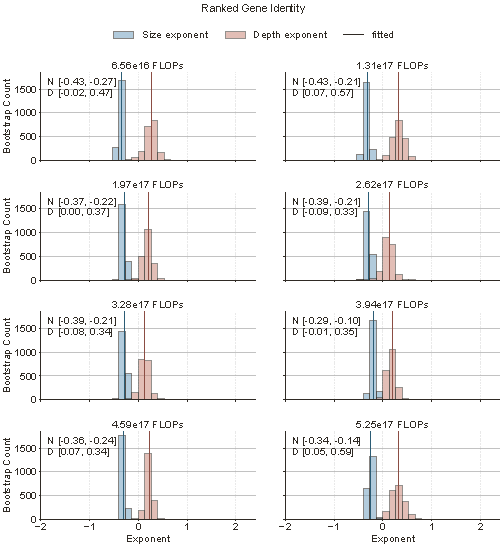
\includegraphics[width=\linewidth]{figures/supp_ranked_lr_bootstrap.pdf}
\end{minipage}\hfill
\begin{minipage}[t]{0.49\textwidth}
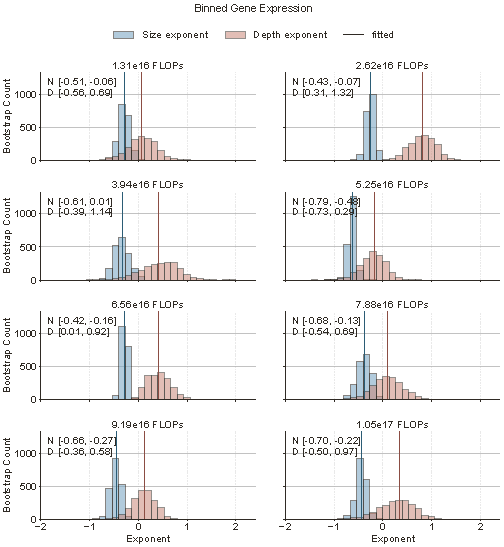
\includegraphics[width=\linewidth]{figures/supp_binned_lr_bootstrap.pdf}
\end{minipage}
\caption{Architecture-resampling sensitivity of the fitted learning-rate exponents. Histograms show exponents from 2,000 bootstrap resamples of the 12 architecture points at each compute slice. Vertical lines mark the fits to the original architecture points; annotated intervals span the 2.5th–97.5th percentiles. These intervals quantify sensitivity to the small sampled architecture grid, not variation over independent training seeds.}
\label{fig:supp-lr-bootstrap}
\end{figure}

\FloatBarrier
\section{Depth-to-width response surfaces}
\label{sec:supp-depth-width}

The depth/width sweep sampled seven depth values at each of seven target parameter counts and evaluated the resulting runs at seven isoFLOP slices.
The response surface models raw loss as a full quadratic in standardised $\log_{10}N$, $\log_{10}C$, and $\log_{10}R$, where $R=D/W$.
Observed isoFLOP profiles remain the primary diagnostic because the fitted optimum is a stationary point of the surface rather than a directly sampled architecture.

\begin{figure}[p]
\centering
\begin{minipage}[t]{0.49\textwidth}
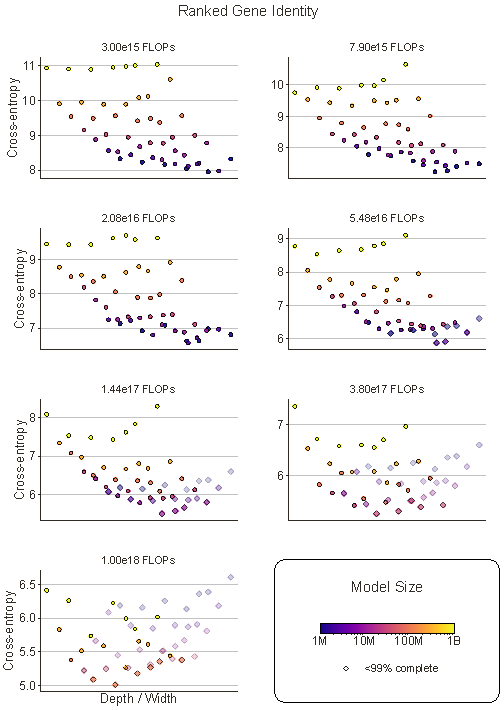
\includegraphics[width=\linewidth]{figures/supp_ranked_dw_observed.pdf}
\end{minipage}\hfill
\begin{minipage}[t]{0.49\textwidth}
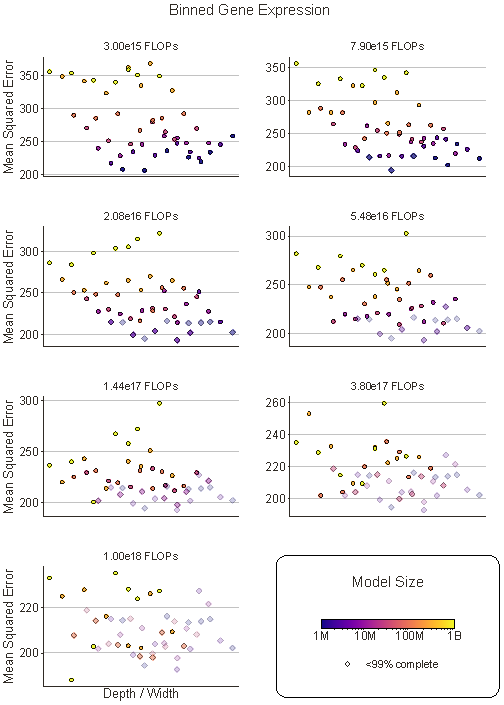
\includegraphics[width=\linewidth]{figures/supp_binned_dw_observed.pdf}
\end{minipage}
\caption{Observed loss as a function of depth-to-width ratio at all seven sampled isoFLOP budgets. Left, cross-entropy for \ranked. Right, mean squared error for \binned.}
\label{fig:supp-dw-observed}
\end{figure}

\subsection{Surface diagnostics and warm-up sensitivity}

Within the prespecified analysis window, the ranked surface fits 256 complete observations with in-sample $R^2=0.987$ and retains $R^2=0.985$ under random five-fold cross-validation and $R^2=0.983$ when leaving out a complete compute slice.
The binned surface fits 230 observations with in-sample $R^2=0.873$ and falls to $R^2=0.864$ and $0.858$ under the corresponding validation schemes.
The side-by-side in-sample diagnostics show substantially greater dispersion and residual variation for the binned surface than for the ranked surface (top row of Figure~\ref{fig:supp-dw-diagnostics}).

To test whether this quadratic description extends into the optimisation transient, we additionally sampled six fixed-compute slices from $10^{14}$ to $1.78\times10^{15}$ FLOPs from the complete training trajectories.
These slices deliberately overlap the architecture-dependent learning-rate warm-up: at the earliest slice, warm-up was still in progress for 49/49 ranked and 38/49 binned runs; even at the latest slice, it was still in progress for 23/49 and 21/49 runs, respectively.
Figure~\ref{fig:supp-dw-slice-windows} places both slice sets on the complete training trajectories and shows the architecture-specific warm-up endpoints.

\begin{figure}[p]
\centering
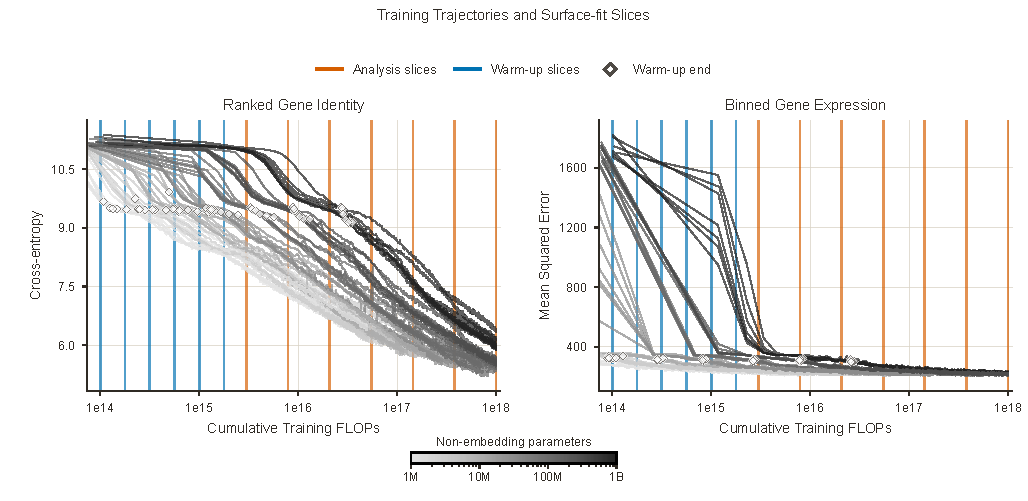
\includegraphics[width=\textwidth]{figures/supp_dw_slice_windows.pdf}
\caption{Training trajectories and compute slices used for the surface diagnostics. Grey curves are exponentially smoothed trajectories for the 49 sampled architectures in each formulation, with shade encoding non-embedding parameter count; diamonds mark the end of learning-rate warm-up for each architecture. Orange lines mark the seven analysis slices used to fit and evaluate the first diagnostic row, while blue lines mark the six warm-up slices used for the second-row extrapolation. The third diagnostic row uses the union of both sets. Left, ranked cross-entropy. Right, binned mean squared error.}
\label{fig:supp-dw-slice-windows}
\end{figure}

We then evaluated the analysis-window surface on these 294 early observations without refitting it.
The ranked $R^2$ falls to $0.376$, while the binned $R^2$ falls to $-0.016$, with large structured residuals (second row of Figure~\ref{fig:supp-dw-diagnostics}).
Thus the quadratic surface is a local summary of the later analysis regime, not a description of the warm-up dynamics; the breakdown is especially pronounced for the binned formulation.
Refitting a single quadratic jointly over all 13 slices improves upon this extrapolation but does not remove the regime mismatch: the combined ranked fit has $R^2=0.972$ over 550 observations, whereas the combined binned fit has $R^2=0.853$ over 524 observations and retains strongly structured residuals (third row of Figure~\ref{fig:supp-dw-diagnostics}).

\begin{figure}[p]
\centering
\begin{minipage}[t]{0.49\textwidth}
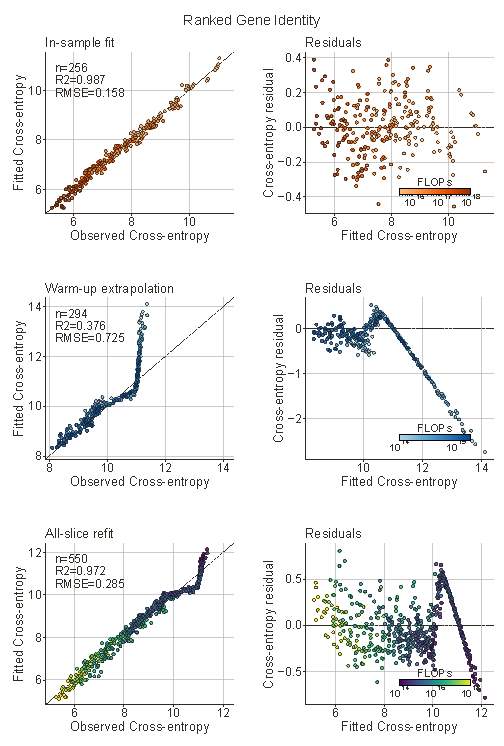
\includegraphics[width=\linewidth]{figures/supp_ranked_dw_fit_diagnostics.pdf}
\end{minipage}\hfill
\begin{minipage}[t]{0.49\textwidth}
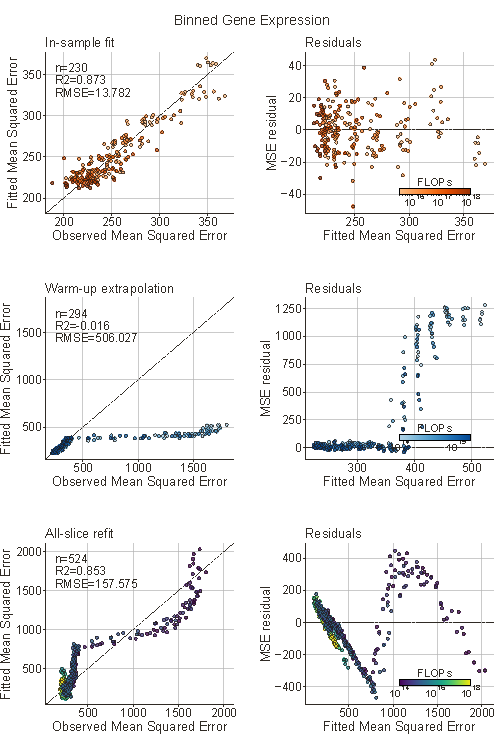
\includegraphics[width=\linewidth]{figures/supp_binned_dw_fit_diagnostics.pdf}
\end{minipage}
\caption{Quadratic-surface diagnostics across the analysis and warm-up regimes. The left group shows \ranked\ cross-entropy and the right group shows \binned\ mean squared error. Within each group, the left panels compare fitted with observed loss and the right panels show residuals against fitted loss. The first row evaluates the surface in sample over the seven-slice analysis window beginning at $3\times10^{15}$ FLOPs. The second row evaluates those same coefficients, without refitting, on six earlier slices from $10^{14}$ to $1.78\times10^{15}$ FLOPs that overlap learning-rate warm-up. The third row refits the quadratic jointly over all 13 slices and displays its residuals over that complete range. Dashed lines mark equality and zero residual; points are coloured by compute.}
\label{fig:supp-dw-diagnostics}
\end{figure}

\subsection{Ranked-model optimum relative to fixed depth}

For the ranked formulation, the fitted optimal ratio scales approximately as $R^*\propto N^{-0.88}$ at fixed compute throughout the plotted domain (Figure~\ref{fig:supp-ranked-ratio-grid}).
This decrease is materially faster than the $N^{-1/2}$ reference obtained by keeping depth approximately fixed while increasing width: because transformer-block parameters scale approximately as $DW^2$, fixed $D$ gives $W\propto N^{1/2}$ and hence $D/W\propto N^{-1/2}$.
The fitted result therefore does not merely recommend holding depth constant as the encoder grows; within this experimental regime it shifts capacity toward width quickly enough that the implied optimal depth itself decreases with parameter count at fixed compute (Figure~\ref{fig:supp-ranked-implied-depth}).

At any fixed parameter count, larger compute budgets shift the optimum upward toward greater depth.
The combined interpretation is conditional: width is favoured as parameter count increases at a fixed compute budget, whereas additional training compute can support deeper architectures at the same parameter count.

\begin{figure}[p]
\centering
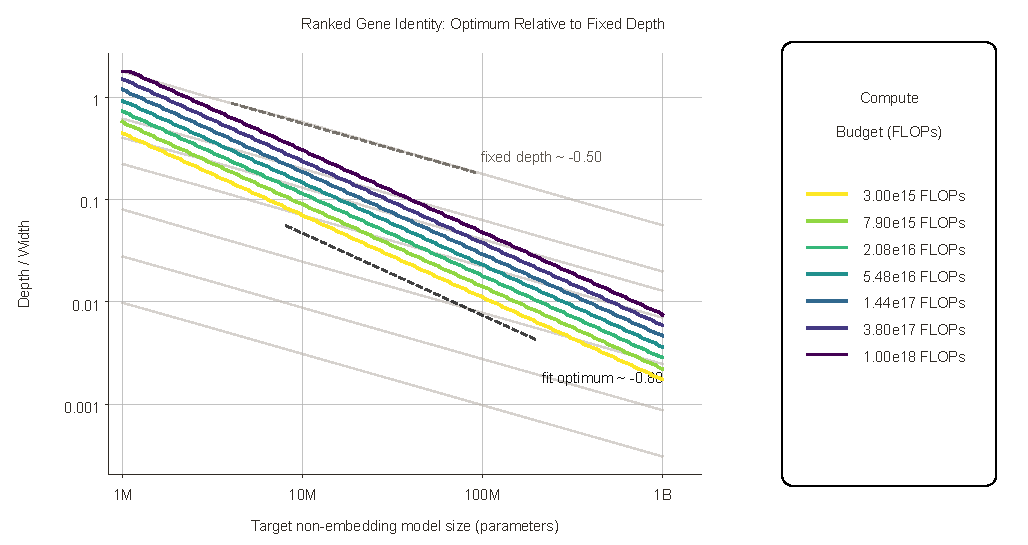
\includegraphics[width=\textwidth]{figures/supp_ranked_dw_ratio_grid.pdf}
\caption{Ranked-model surface optimum against the sampled fixed-depth ratio grid. Grey lines show the ratios generated by fixed depths; coloured lines show the fitted optimum at seven compute budgets. Dashed guides compare the approximate $-0.50$ fixed-depth slope with the fitted $-0.88$ slope in log--log space.}
\label{fig:supp-ranked-ratio-grid}
\end{figure}

\begin{figure}[p]
\centering
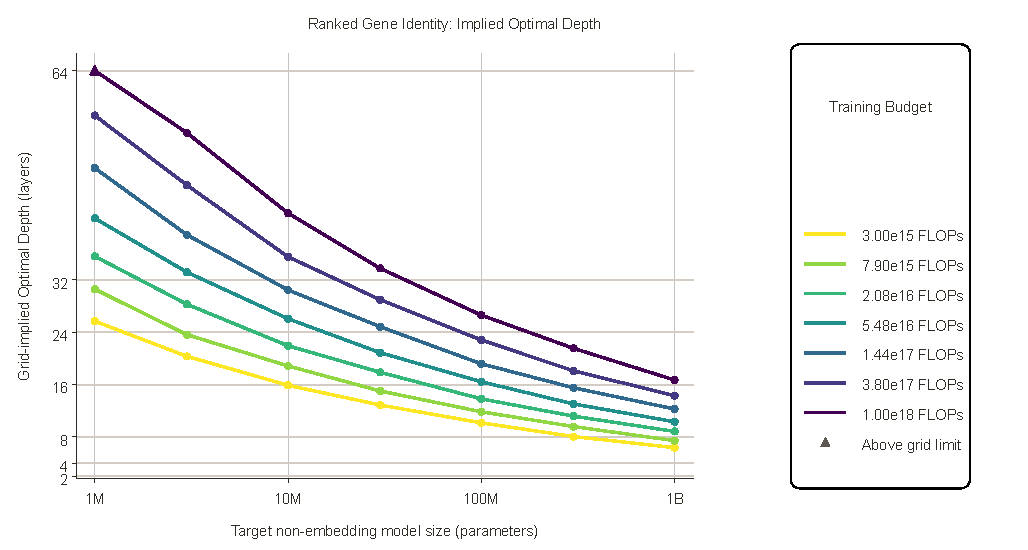
\includegraphics[width=\textwidth]{figures/supp_ranked_dw_implied_depth.pdf}
\caption{Grid-implied ranked-model optimal depth. The loss-minimising ratio is selected within the observed ratio range and mapped back onto the sampled depth/width grid by interpolation in log space, with values outside the grid at a given parameter count clamped to its depth limits. Circles denote interior estimates; triangles mark boundary-limited values where the unconstrained surface optimum lies beyond the supported range, with direction indicating the exceeded limit. In particular, the depth-64 point at 1 million parameters and $10^{18}$ FLOPs is an upper grid limit, not an identified unconstrained optimum. At fixed compute, the implied depth decreases as the target parameter count increases; at fixed parameter count, it increases with the compute budget.}
\label{fig:supp-ranked-implied-depth}
\end{figure}

\subsection{Uncertainty in the binned-model architectural optimum}

Predictive error alone is not the decisive limitation.
The binned stationary point is less precisely determined under row-bootstrap resampling: 4 of 250 fitted surfaces (1.6\%) are non-convex in the log-ratio direction and therefore do not define a minimum.
Even among the convex binned fits, the central 95\% interval of the inferred optimum at 100 million parameters and $10^{18}$ FLOPs spans approximately 1.79 orders of magnitude (a factor of 62).
By contrast, all 250 ranked bootstrap surfaces are convex and their inferred optima span approximately 0.42 orders of magnitude (a factor of 2.6) at the same reference point.
These central 95\% intervals use the 2.5th and 97.5th percentiles, whereas the bands in main Figure~5 use the 5th and 95th percentiles.
Rows from the same training run are correlated, so these are surface-sensitivity diagnostics rather than independent-run confidence intervals.
The binned surface has lower held-out predictive accuracy and a broader optimum interval than the ranked surface. We therefore treat its stationary point as a less precise descriptive estimate and do not prescribe an optimal $D/W$ rule from it.

\FloatBarrier
\section{Implementation details, limitations, and priority checks}
\label{sec:supp-limitations}

\subsection{Binned loss conventions across experimental stages}

The binned context-length/model-size and learning-rate sweeps used expression MSE over masked positions for which the activity head predicted a probability greater than 0.5.
The binned batch-size and depth/width sweeps instead selected masked positions whose target expression bin was non-zero.
Thus prediction-selected MSE can include masked zero-expression targets classified as active and omit masked non-zero targets classified as inactive.
The selected sets, and hence their expression losses, coincide when all masked activity classifications agree with the targets.
High activity-prediction accuracy supports substantial overlap, but does not establish identical MSE values because discrepancies also depend on the squared expression errors at the differing positions.
The analyses retain the selection convention used in each sweep; no paired estimate of the effect of changing that convention is reported here.

For the context-length/model-size and learning-rate sweeps, activity BCE was computed after setting both the logits and targets to zero at unmasked positions, summing over all positions, and dividing by the number of masked positions.
Let $T$ be the number of sequence positions in a minibatch, $M$ the number masked, $z_i$ the activity logit, and $a_i=\mathbf{1}[x_i>0]$ the activity target. For $M>0$, the recorded term is
\begin{equation}
 L_{\mathrm{act,recorded}}
 = \frac{1}{M}\sum_{i\in\mathcal{M}}\operatorname{BCEWithLogits}(z_i,a_i)
   + \frac{T-M}{M}\ln 2.
\end{equation}
The second term depends on the sampled mask but not on model parameters, so it contributes no parameter gradient.
It affects the numerical activity-loss value, whereas the expression-loss selection convention can affect both the expression metric and training gradients.
In the batch-size and depth/width sweeps, the activity loss was averaged directly over masked positions, without the unmasked-position contribution.
The paper's binned scaling figures use the expression-loss component throughout.

\subsection{Other implementation and evaluation considerations}

The ranked input pipeline pads cells with fewer expressed genes than the requested context length.
In the original ranked sweeps, transformer attention and mean pooling did not explicitly exclude padded positions.
The later completion of the missing ranked architecture used padding-aware attention; pooling still averaged over the full sequence length.
At context 256 the expected exposure is limited because typical cells contain more expressed genes and are truncated, but this expectation does not replace a representative rerun with explicit padding masks.

In the binned context-length/model-size, learning-rate and batch-size sweeps, the input constructor requested expressed and unexpressed genes using separate floor operations.
For those sweeps, the effective sequence length is one position below the nominal value, so the nominal-context FLOP estimator slightly overstates compute relative to the positions processed.
The replacement binned depth/width sweep used the corrected constructor, preserving all 256 positions and excluding padding from both masking and attention.
These implementation variants were checked against the archived implementations used to deliver the experiments; the publication recipes identify the behavior modes and accompanying standalone reference tests.

The validation cell identities are fixed, but gene selection and masking are resampled at each validation event.
Representation evaluation uses selected but unmasked inputs, so checkpoint-to-checkpoint variation includes stochastic gene selection.
Finally, the architecture sweeps do not contain independent training-seed replicates.
The most informative next checks are therefore targeted rather than exhaustive: repeat representative small, medium, and large architectures across seeds; repeat validation embedding inference; compare the implemented ridge probe with centred and standardised variants; test alternative coarse-taxonomy resolutions; and replace the row bootstrap with a cluster bootstrap over complete architecture runs.

\section{Software and reproducibility records}

The pipeline used Python 3.12, PyTorch \texttt{2.11.0+cu128}, Lightning 2.6.1, TileDB-SOMA 2.3.0, TileDB-SOMA-ML 0.1.0, Scanpy 1.11.5, and scIB 1.1.7.
Float32 matrix-multiplication precision was set to \texttt{medium} and training used bfloat16 mixed precision.
Each task used one NVIDIA accelerator: either an RTX PRO 6000 Blackwell GPU with 96~GB or an Ampere A100 GPU with 64~GB.


\end{document}
